\chapter{Pointing Experiment}
\label{chap:pointing}

This chapter was originally published in the conference proceedings for AIAA Modeling and Simulation Technologies 2015.

\section{Introduction}

The underlying motivation for this project is to bring high-fidelity simulator response to an earlier stage in the cockpit design cycle, where traditionally, the focus is on layout of displays and controls in a minimally-functional mockup.
With the R3C concept, system functionality can be experienced from the start, in the virtual environment via a head-mounted display (HMD), while the user interacts with the cockpit systems by touching the surfaces of a low-fidelity (3-D printed) environment.
The user receives the tactile feedback of touching a button or edge-key, and via hand-tracking technology, sees the response in the virtual displays.
Required changes to the user-interface environment or even ``what-if'' ideas can be made quickly and at low cost by modifying the 3-D printed surfaces, and then reflecting these physical changes in the virtual visual scene.
By creating a high-fidelity virtual simulator on top of a low-fidelity geometric mockup, this approach may allow more design/layout iterations at lower cost, which could lead to a final design that is closer to optimum than would be feasibly attained with traditional approaches.

We have developed a proof of concept of the R3C system, which was used to perform an initial, simple, targeting study to validate our approach, and which will be the basis for future work.
Figure \ref{fig:pe_prototype} shows an over-the-shoulder view of a user of the R3C prototype with annotations to call out the major components of our current technical approach.
The user is wearing an immersive virtual reality head mounted display (Oculus Rift Development Kit 2), which presents them a virtual scene (shown in Figure \ref{fig:pe_virtual}) that is spatially stabilized with respect to the physical instrument panel.
As the user reaches out toward the inert 3D printed instruments, a LeapMotion hand tracker reads the position of each finger and the pose (attitude and configuration) of the hand.
A simple collision detection algorithm, described below, uses this information to determine when a user has touched a button.
Since it is important for the user to visually track their own hand during pointing and actuation tasks, we also use the hand tracker to render the dynamic position of the hand in the virtual scene (Figure \ref{fig:pe_virtual}).
On certain buttons we have added copper pads that are connected to a capacitive touch sensor as a secondary sensor for button actuation.
The camera mounted above the panel is an infrared camera that senses the position of the HMD.
The display on the screen can be configured as desired; it is currently showing an external camera view.
The behaviors of each button are controlled in software, and can be easily reconfigured.

\begin{figure}
    \centering
    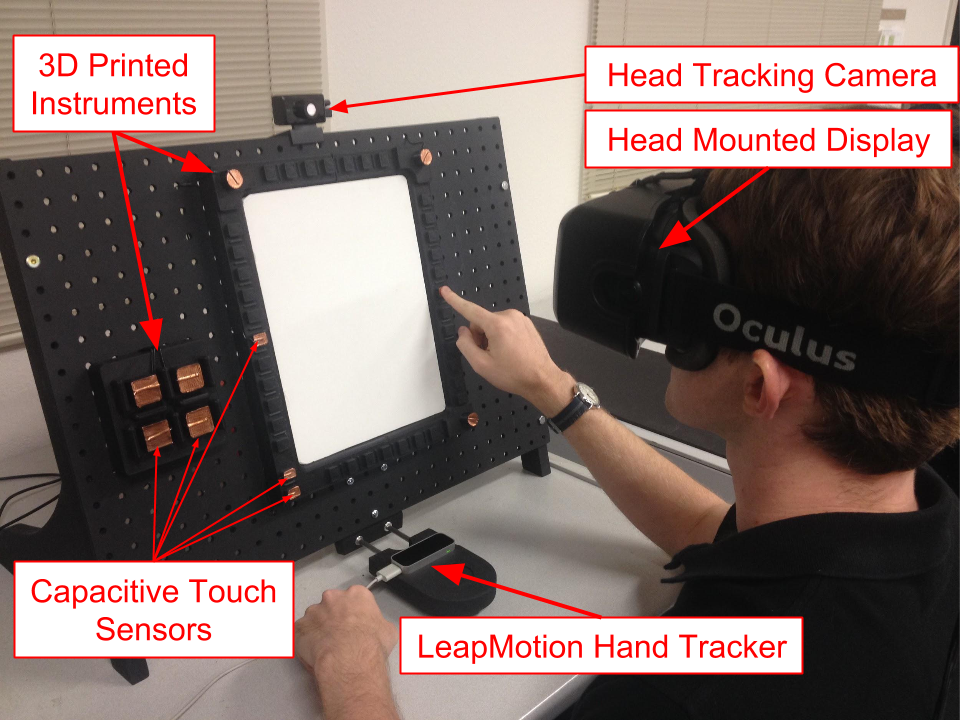
\includegraphics[width=4.0in]{pe_prototype.png}
    \caption{Prototype R3C System}
    \label{fig:pe_prototype}
\end{figure}
\begin{figure}
    \centering
    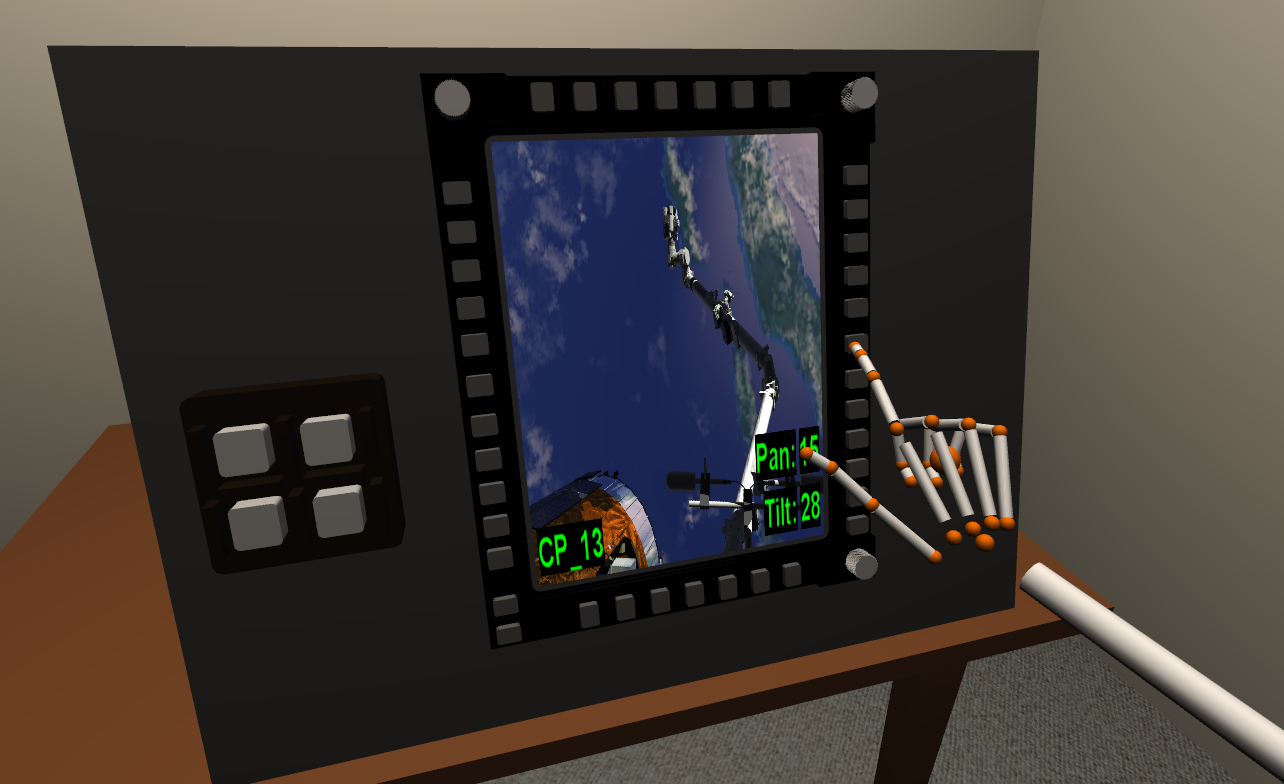
\includegraphics[width=4.0in]{pe_virtual.png}
    \caption{Virtual view of user from Figure \ref{fig:pe_prototype}}
    \label{fig:pe_virtual}
\end{figure}

The use of virtual or augmented reality in aerospace has been extensive, starting with the first flight simulators, and even in the cockpit in research studies\cite{foyle_taxiway_1996, bachelder_fused_2013}.
Significant recent work investigates virtual reality tools in a simulator\cite{h._wan_mrstudio:_2011, i._yavrucuk_low_2011, t._aslandere_virtual_2015}.
However, our concept of merging an accurate but low-cost tactile environment with the high-fidelity virtual view is so far untested.
Accurate haptic feedback has been a goal of virtual reality (VR) researchers since the emergence of VR.
Providing dynamic haptic feedback, however, still proves challenging to date\cite{stone_haptic_2001,lecuyer_simulating_2009}.
Our approach allows accurate haptic feedback for the case of a static workstation, such as found in a real cockpit.
Combined with 3D printing and our virtual simulator overlay, this provides an inexpensive platform to create a functioning simulator, able to adapt quickly to large-scale design changes.

\section{Technical Approach}

This section details the components of our prototype and how they are integrated into the R3C system, as well as rational for selection, improvements and lessons learned.

\subsection{3D Printed Instruments}

A central tenant of our technical approach is to use physical, geometrically accurate instrument shapes that provide no functionality (i.e.\ no screens, no working buttons, etc.).
This is intended to imitate the fidelity of a typical early design stage mockup.
In order to achieve this we have produced 3D-printed ``instruments'' that can be easily rearranged on a panel mount (pegboard).
Since the devices are rapidly prototyped, they can be redesigned in a much smaller time frame than typical simulator instruments.
By using the geometrically accurate instruments at the correct cockpit locations, the user is provided with accurate tactile and proprioceptive feedback without the need for entering the challenging field of virtual haptic feedback.

\subsection{EDGE Rendering Engine}

We are using a NASA developed rendering engine named EDGE8 to provide the visuals for the virtual scene rendered in the head-mounted display (HMD).
EDGE is highly customizable and extendable through C/C++ plugins, Tcl scripts, or networking functions.
Existing dynamic simulations (e.g. Matlab) can also be integrated.

\subsection{Oculus Rift}

The Oculus Rift virtual reality head mount display is currently only available as a developer kit.
The lightweight headset provides an immersive virtual reality experience by combining a wide field-of-view scene with accurate head tracking, giving a stable virtual world.
The small display (cell phone sized) is viewed through a single set of lenses, and the barrel distortion of the lens is corrected for in the rendering engine by a pincushion distortion of the rendered scene.
The orientation of the head is tracked using internal sensors as well as an infrared camera to give an accurate pose for rendering the scene.
The software developer’s kit9 (SDK) exposes the head position and orientation and provides the appropriate distortion for a rendered scene (which is done for each eye), and this has been developed into an EDGE plugin.
The technology of these head mounted displays is improving rapidly, driven by technology developed for the cell phone and demand from the gaming industry.

The head tracking provided in the newest development kit version gives a significant improvement over the original Oculus Rift in the registration between the real world and the virtual world.
The head-tracking camera is mounted on a known location on the panel (see Figure \ref{fig:pe_prototype}), and the tracking software provides a measurement of the relative location between the head and the camera.
The virtual world can then be rendered relative to the location of the camera.


\subsection{LeapMotion Hand Tracker}

The LeapMotion hand tracker is a small, consumer orientated optical hand tracker.
It uses two infrared cameras as the source of its proprietary tracking algorithm.
As of version 2.0 of their SDK10, they expose to the application developer the positions of all the joints and bone positions of the hand.
An EDGE plugin was developed in-house at UC Davis to position the nodes in the scene from this information, which is the source for rendering the virtual hand as well as the button detection algorithm.

We decided to use the LeapMotion as it provides logistical simplicity compared to professional motion capture devices that require multi-camera setups with lengthy calibrations as well as high cost.
A main goal of our system is that it can be used without much setup in the physical world, leading us to the new small optical trackers.
There are other promising devices (i.e. Kinect2 and other 3D camera systems) that could be used in the future.

\subsubsection{LeapMotion Calibration}

Early in the integration process, we discovered that the LeapMotion provided precise and repeatable measurement of the hand positions throughout its tracking volume.
The accuracy as the hand got further away from the sensor, however, was insufficient.
Put another way, the position of the hand in the virtual world was offset from the true button position in the physical world, yet the offset was consistent between movements.
This led us to develop a calibration to provide a more accurate registration between the virtual and physical hand positions.
Since we accurately know the position of the panel and instruments, it is only required to solve the following linear algebra equation for the transformation matrix, $\mathbf{T}$:
\begin{equation}
    \vec{x}_{known} = \mathbf{T}\vec{x_{measured}}
    \label{eq:pe_Tvec}
\end{equation}

Using a simple least squares approach to find the coefficients of the matrix, the registration between the virtual and physical worlds is vastly improved.
The transformation matrix is not constrained to a simple rotation (i.e.\ not assumed orthogonality or other special properties) so the solution is found by expanding and solving the general homogenous coordinates transformation matrix.

\begin{equation}
    \begin{bmatrix}
        x_{known} \\
        y_{known} \\
        z_{known} \\
        1
    \end{bmatrix} =
    \begin{bmatrix}
        T_{11} & T_{12} & T_{13} &T_{14} \\
        T_{21} & T_{22} & T_{23} &T_{24} \\
        T_{31} & T_{32} & T_{33} &T_{34} \\
        0 & 0 & 0 & 1
    \end{bmatrix}
    \begin{bmatrix}
        x_{measured} \\
        y_{measured} \\
        z_{measured} \\
        1
    \end{bmatrix}
    \label{eq:pe_Tmat}
\end{equation}

Typical least squares approaches would attempt to find $\mathbf{x}_{measured}$ in Eqn.\ \ref{eq:pe_Tvec}, however we desire to find the matrix T itself.
It can be shown that expanding the matrix equation (Eqn.\ \ref{eq:pe_Tmat}) for multiple points (i.e.\ $\vec{x}_{known,1},\dots,\vec{x}_{known,n}$ and $\vec{x}_{measured,1},\dots,\vec{x}_{measured,n}$) and then collecting like terms will convert the problem into three different least squares problems.
They are shown here, dropping the subscripts to $k$ and $m$ for known and measured.

\begin{gather*}
    \begin{bmatrix}
        x_{k1} \\
        x_{k2} \\
        \cdots \\
        x_{kn}
    \end{bmatrix}
    =
    \mathbf{X}_M
    \begin{bmatrix}
        T_{11} \\
        T_{12} \\
        T_{13} \\
        T_{14}
    \end{bmatrix}
    ,\;\;
    \begin{bmatrix}
        y_{k1} \\
        y_{k2} \\
        \cdots \\
        y_{kn}
    \end{bmatrix}
    =
    \mathbf{X}_M
    \begin{bmatrix}
        T_{21} \\
        T_{22} \\
        T_{23} \\
        T_{24}
    \end{bmatrix}
    ,\;\;
    \begin{bmatrix}
        y_{k1} \\
        y_{k2} \\
        \cdots \\
        y_{kn}
    \end{bmatrix}
    =
    \mathbf{X}_M
    \begin{bmatrix}
        T_{31} \\
        T_{32} \\
        T_{33} \\
        T_{34}
    \end{bmatrix}
    ,\\
    \text{where}~\mathbf{X}_M =
    \begin{bmatrix}
        x_{m1} & y_{m1} & z_{m1} & 1 \\
        x_{m2} & y_{m2} & z_{m2} & 1 \\
        &\dots & & \\
        x_{mn} & y_{mn} & z_{mn} & 1
    \end{bmatrix}
\end{gather*}

At least 4 points are needed to solve this system, and it has been found that a calibration with small least squares residuals can be achieved with 10-20 well chosen points.
The panel and instrument edges can provide well-known points, as well as button locations.
The calibration matrix is then used to find the offset of the tip of the index finger for  each hand, and this offset is used to move the entire hand.

\subsubsection{LeapMotion Mounting Position}
The LeapMotion software recently (as of version 2.2) began officially supporting a ``VR Mode'' which allowed users to mount the device on the front of a VR HMD and track the hands relative to the head.
This was tested in our system and although we experienced better tracking, the hand would not stay stable relative to the panel during head movement.
This led us to develop a mount that would hold the LeapMotion above the panel looking down, and putting the software in ``VR Mode'' we were able to achieve better tracking but with a fixed known position, the hand remained stable relative to the panel.

\subsection{Button Detection Algorithm}
\label{sec:pe_button}

The button detection algorithm is a simple collision detection model.
A rectangular box is defined that extends outside the button, including a tolerance zone to account for misalignment and poor tracking.
When a fingertip enters and stays in the box for 50ms then a button event is triggered.
An event is also triggered when a finger enters the box, which we use to change the color of the button to indicate proper alignment to the user.
The advantage to using the optical tracking to determine when a user has selected a button is that it has the potential to significantly reduce the complexity of the system.
If the pilot interactions with the panel can be determined solely by tracking his/her hands from the external sensor, then the cockpit panel needs only to provide physical feedback, and does not require any wiring.
Of course, the primary drawback of this approach is that the efficacy is limited to the accuracy and reliability of the hand tracker, and the algorithms tracking this movement for button inputs.
Nonetheless, as we show in our experiment, the LeapMotion coupled with this algorithm can be used effectively.

For the experiment described below, the collision detection box was set to extend 0.5 inches inward and outward from the button, including a 0.1-inch tolerance on all dimensions.
Aslandere \cite{t._aslandere_virtual_2015} found no significant effect with button selection ability based on changing this volume in a purely virtual environment, so we did not change the collision detection box size for this first test of the R3C (although it is easily modified in software).

\subsection{Capacitive Touch Sensors}

For this early research phase, we needed a baseline method to determine if a button was touched, for comparison with the LeapMotion IR camera hand tracking method.
A simple method was first developed using copper tape electrodes on top of certain buttons (as can be seen in Figure \ref{fig:pe_prototype}).
These electrodes are connected to a Freescale MPR121 capacitive touch controller that registers when a finger touches them.
The capacitive touch controller is connected to an Arduino, acting as a serial communicator between the microchip and the computer.
This setup provides a binary state of whether a finger is touching the button.
This is used to help determine whether the button detection algorithm using the hand tracker is working correctly.

Since touch accuracy can be important in safety-critical applications, we also desired the ability to record where on the button the finger press was located.
This would help to determine if we had any registration biases in our system.
To accomplish this, a custom printed circuit board was developed that provides an electrode array of 5 rows and 5 columns over a 1-inch by 1-inch square.
This board is show in Figure \ref{fig:pe_capacitive}, where it is mounted in a 3D printed instrument.
The capacitive state of each row and column can provide a measurement of the center of the finger press on the grid created by the rows and columns.
With this configuration finger-location accuracy of under 0.1-inch can be achieved.
The location of the finger press can help provide a measure of the accuracy of the registration between the optical sensors and the real world location.

\begin{figure}
    \centering
    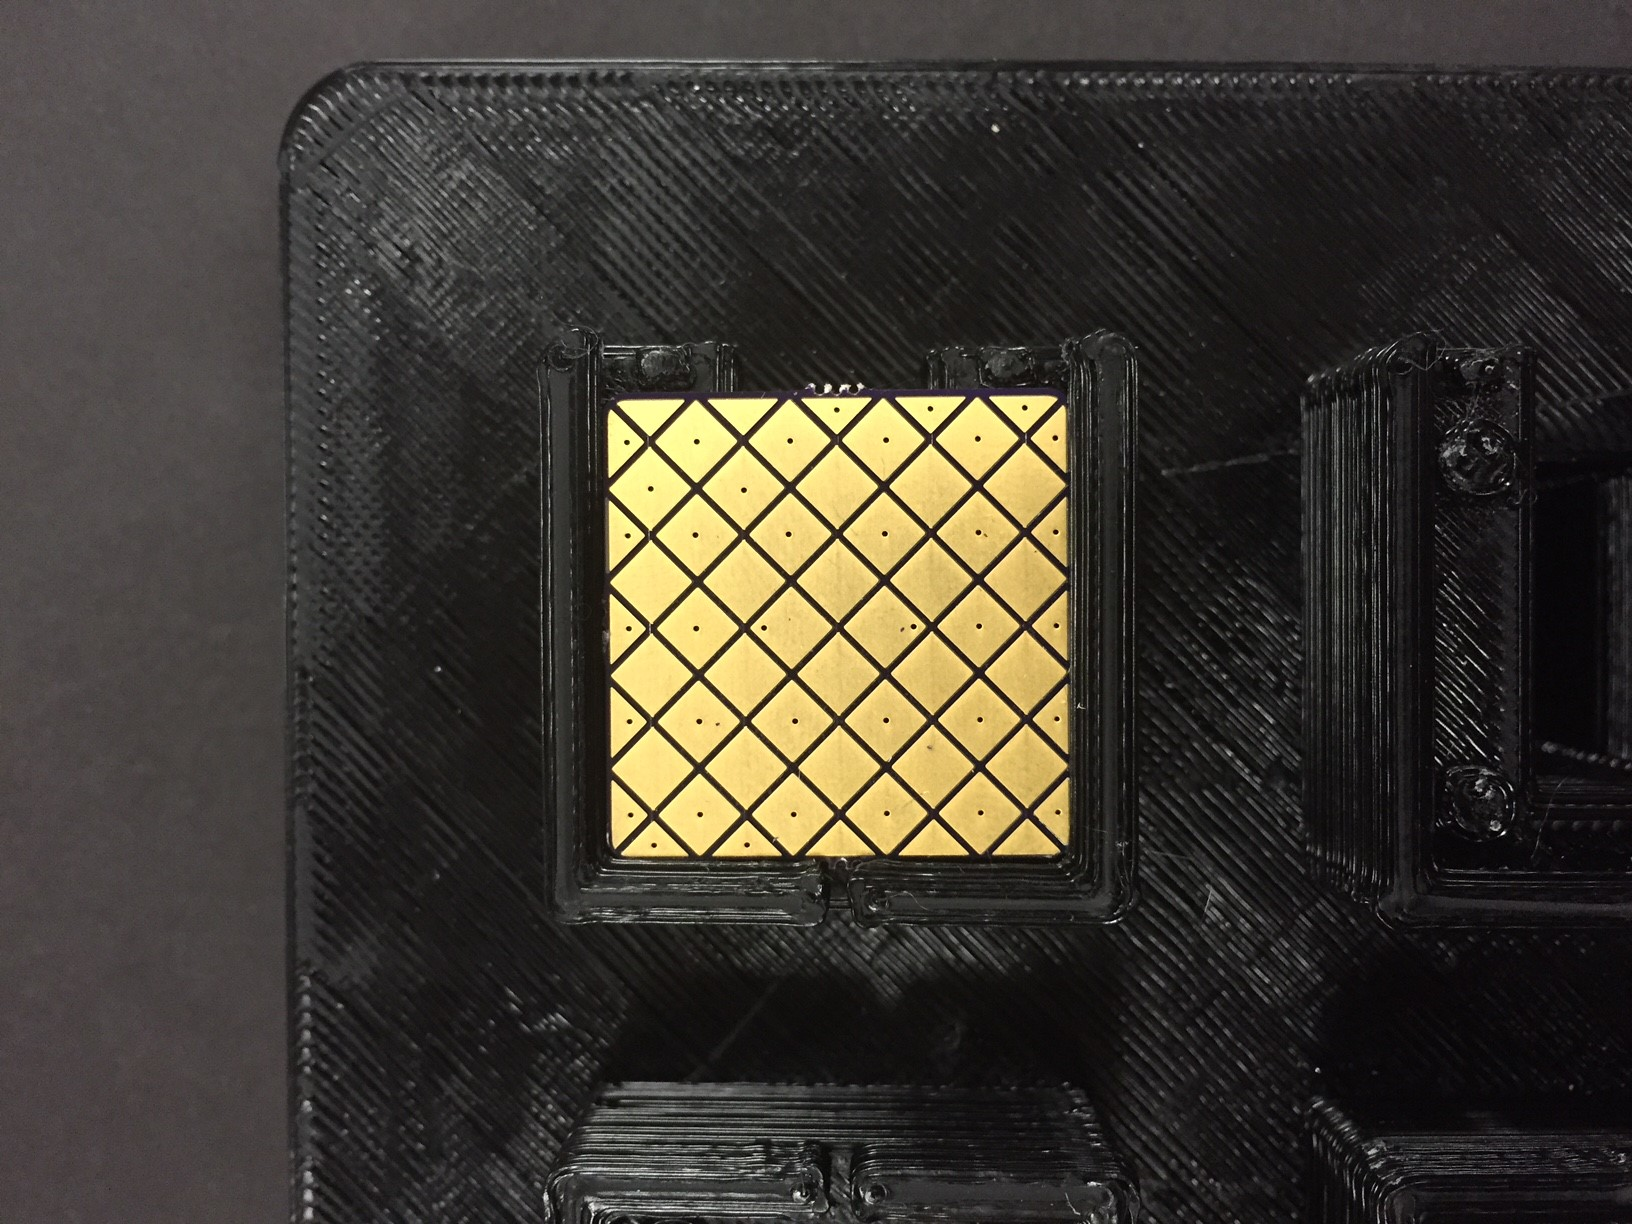
\includegraphics[width=1.25in]{pe_capacitive.jpg}
    \caption{Capacitive touch array button. Each row and column of diamond pads are connected as one electrode each and together can provide location information of where the user presses.}
    \label{fig:pe_capacitive}
\end{figure}

\subsection{Summary and Lessons Learned}

We've discovered a few qualitative effects of various technologies and methods throughout the time we’ve spent building this prototype, resulting in the following ``lessons learned''.

The registration between the virtual world and real world was a concern in the first prototype that did not include the head tracking setup of the Oculus Rift DK2, and it required precise measurement between the location of the user (including seat height) and the desk and panel.
This would cause problems when the head orientation yaw sensors drifted as well, where the user would not be lined up with the panel after a few minutes of use.
The upgrade to the head-tracking camera to anchor the virtual world to the real world greatly improved the both stability and accuracy, and also significantly improved the feeling of presence in the virtual environment.

The registration between the real world and the hand tracker position in the virtual world is even more important, however.
Since the user can feel the proper place for their finger when the finger arrives at the target, if the hand tracker is not lined up they may not be able to activate the button detection algorithm easily, or at all if there is physical interference.
This problem created the need for the calibration scheme, and having the calibration is essential for using the LeapMotion in a task where the real and virtual world needs to be aligned.
This problem also highlights the importance of testing people who are new to the system.
New users were fixated on placing their finger where the physical feedback indicated the button was and did not adjust for misalignments with the hand tracker, while expert users learned to ignore the physical feedback and activated the hand tracker by finding the misaligned location.
Additionally, we discovered that hand pose and speed can influence the performance of the hand tracker, such that expert users can perform in the system quicker and with greater accuracy.
This is discussed again later in the context of the experiment performed.

The purely optical button detection algorithm is prone to failures, especially without a complex algorithm performing heuristics on the movement to determine the users desired selection.
The simple collision detection model works well, but is difficult for the user without the loop-closing visual indication of when the detection box is activated.
In our case we added the button changing color.
It was also important to have a slight delay in activation, as this not only provides a failsafe for false positives, but it also adds a way to explore the tactile surface without consequences.

The latency of the entire R3C system has not yet been quantified, and there are two significant aspects where this might be interesting: from hand movement to hand tracker measurements through the rendering pipeline to the image shown to the user; as well as from head movement through to the image shown to the user.
However, latency is clearly low enough to make measuring it low priority, as the hand movement delay in the virtual world is unnoticeable to the average user.
Additionally, the latency of the Oculus Rift head mounted display is drastically improved from earlier technologies such that it does not cause a concern.
Finally, the manufacturers of both LeapMotion and Oculus are actively improving on the latency on both fronts.

We also initially found tracking performance degradation when the finger approaches the instrument panel that was due to optical interference with the panel objects (i.e.
it was happening only when the panel was present).
This was improved when we moved the LeapMotion to the top looking down, but the larger effect was found when looking at the image captured by the LeapMotion infrared cameras, discovering our black 3D printed instruments were highly reflective in infrared and showing up the same color as the hand.
Applying a matte finish greatly improved this, but it is still a problem we are dealing with to date.
We have also found better results when controlling entire backdrop of the LeapMotion field of view with a dark matte material, as this helps provide a greater contrast between the hand and the background.
There still remains work to improve this, as a few subjects in the experiment indicated they found degraded tracking with the panel present.

\section{Experimental Methods}

\subsection{Experiment Goals and Motivation}
We performed a brief pilot study to validate our technical approach and take some measurements of the effects of using the R3C system.
Specifically, we were interested whether a new user could accurately target the correct button in an instrument panel, and how the different technologies used affected the targeting task.
There were three main effects of the targeting task under study in this experiment:
\begin{itemize}
    \item The effect of the use of the VR HMD versus no VR HMD (i.e.\ virtual vs.\ real world).
    \item The effect of the physical panel versus no physical panel present\ (i.e.\ having the tactile feedback vs.\ no tactile feedback)
    \item The effect of the optical tracking button detection versus the capacitive touch button detection
\end{itemize}
The use of the virtual reality headset also implies that subjects have to rely on the visual feedback from the hand tracker virtual hand to target the button.

We were concerned about the effect of both touch-selection accuracy and movement time, but the context for our design is an aerospace cockpit, where accuracy in selecting the intended button is typically paramount over movement time.
Previous research in targeting tasks in virtual environments has not always reported on success rates, indicating incorrect trials were re-performed.
We did not do this, as we wanted to ensure we recorded the success rate.

Previous work has investigated various 3D pointing tasks in the real and virtual world without tactile feedback\cite{liu_comparing_2009}, or with tactile feedback but no immersive virtual reality\cite{teather_evaluating_2010}, or with virtual haptic feedback\cite{chun_evaluating_2004}, or pure virtual worlds\cite{bruder_touch_2013,grossman_pointing_2004}.
Our work differs in the use of the tactile feedback provided by the panel combined with an immersive virtual world.

\subsection{Experiment Design}

Figure \ref{fig:pe_diagram} shows a diagram of the experimental setup.
The panel was configured with a single four-button keypad, arranged in a 2x2 grid.
Three different starting pads were placed on the desk near the edge.
The buttons on the keypad were $1^{\prime\prime} \times 1^{\prime\prime}$ and were equipped with the capacitive touch sensor arrays as described above, allowing the measurement of position of finger press.
The start pads were capacitive touch copper tape electrodes, also $1^{\prime\prime} \times 1^{\prime\prime}$, but had no position detection capability.
The participants were asked to start with their index finger on the proper start pad and then target the correct button on the panel.
Audio prompts were given through headphones, which indicated the starting pad and panel button goal before each task.
Subjects were instructed to target the center of the correct button, but were given no instructions on speed.
Subjects targeted the button using their index finger of their dominant hand, which was the right hand for all subjects.
Each participant performed 48 targeting tasks under each of the four different conditions:
\begin{enumerate}
    \item  Wearing the HMD, button selection registered by capacitive sensors, panel physically present
    \item Wearing the HMD, button selection registered by hand tracking sensors, panel physically present
    \item Wearing the HMD, button selection registered by hand tracking sensors, panel not physically present
    \item Not wearing the HMD, button selection registered by capacitive sensors, panel in position
\end{enumerate}
Before each condition the subjects were given one set of 12 trials for familiarization of that particular condition.
During the ``no panel'' condition, the hand tracker remained mounted at the same point, but the panel was moved out of the way, such that the subjects were targeting the buttons in the virtual world only.
The button selection in every condition was indicated by a sound played in the headphones when the appropriate sensor measured a button press.
In addition, during the optical sensor trials, the button color changed color to indicate they had entered the selection zone (as described in Section \ref{sec:pe_button}).
The tasks would time out after 10 seconds.
The task was not repeated for an incorrect button selection or timing out, instead the subject moved on to the next task.
The condition order was randomized for each subject, and the tasks were performed in a pseudo-random order.

\begin{figure}
    \centering
    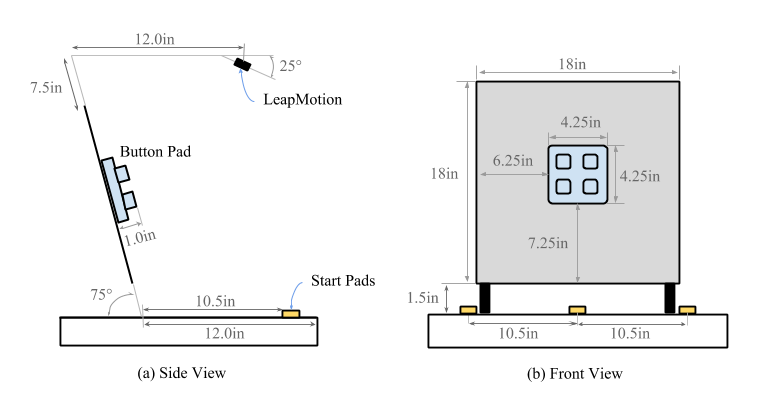
\includegraphics[width=\textwidth]{pe_diagram.png}
    \caption{Diagram of Experiment Setup}
    \label{fig:pe_diagram}
\end{figure}

The subjects were all briefed on the technology from a prewritten speech explaining how to activate each of the sensors.
No information was given on how to best perform the task or advice on working with the various sensors.

The dependent variables measured were time from starting pad to trial goal button, accuracy measured on the capacitive touch sensors (except for condition 3 where this was not possible), as well as success rate.
The raw data from the LeapMotion hand tracker was also recorded for each trial, allowing for post analysis of hand trajectory.

\subsection{Subject Pool}
The experiment was performed with 8 subjects, recruited from the university student population, all with no or limited previous exposure to the R3C setup.
All subjects indicated they had either never used a virtual reality headset or briefly tried them once or twice.
Ages ranged from 18-31 with 6 male, 2 female.
They all had correctable vision to 20/20 and none indicated difficulty seeing the image in the virtual reality HMD.
After the experiment, every subject indicated no motion sickness, and only mild eyestrain was reported.

\section{Results}

The time was recorded for each trial from release of starting pad to the successful button press using the correct button registration.
Trials which timed out or where the incorrect button was targeted were discarded for the time analysis.
The time for each trial was corrected for the varying distances of the movements by multiplying by the average distance (18.4 in) over the straight-line distance between the start and goal button for that trial (which varied from 15.5in to 20.5in).
A boxplot of the distribution of the corrected time grouped by condition across subjects is shown in Figure \ref{fig:pe_boxplot}.
The effects of each were determined using a two sample T-test on the corrected time measure between the appropriate conditions.
The effect of the use of the HMD between condition 1 and 4 (both using capacitive and panel) was significant (p < 0.01), and on average caused the corrected time to drop 1.31 seconds.
The optical detection algorithm also has a negative effect on corrected time (p < 0.01), comparing conditions 1 and 2, but the drop in performance was only 0.55 seconds.
However, it was found that the panel had no significant effect on performance across all subjects (conditions 2 and 3).

\begin{figure}
    \centering
    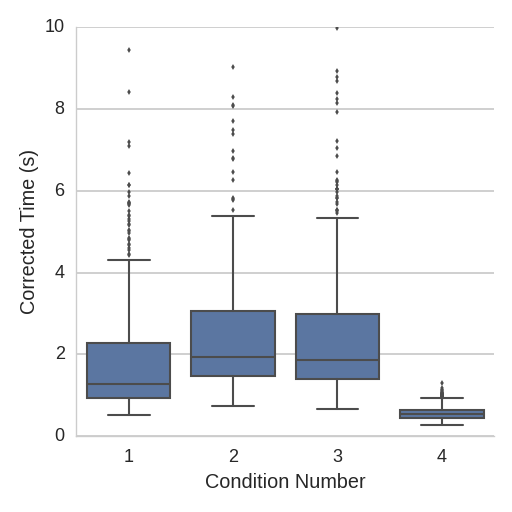
\includegraphics{pe_boxplot.png}
    \caption{Boxplot of normalized time distribution by condition. Condition numbers are: 1. HMD, Capacitive, Panel; 2. HMD, Optical, Panel; 3. HMD, Optical, No Panel; 4. No HMD, Capacitive, Panel. The median is indicated by the line in the box, the boxes contain the inter-quartile range (IQR), and the whiskers extend to 1.5*IQR with outliers plotted.}
    \label{fig:pe_boxplot}
\end{figure}

\begin{table}
    \centering
    \includetable{pe_results}
    \caption{Mean results across subjects. Standard deviations are reported as $\sigma$.}
    \label{tab:pe_results}
\end{table}

When comparing the results of the corrected time within subjects it was found that 3 subjects had a significant positive effect with the panel while only 1 subject had a significant negative effect, the rest showing no effect.
Similarly, the optical tracking versus capacitive tracking had no effect on 3 subjects, while the rest display the same as the between subjects finding of negative effect.

The selection of the correct button was performed almost without error, which is a promising result for new users of the system.
There was no significant effect between the different conditions on success rate.
Over 8 subjects and 1517 trials, only 12 trials selected the wrong button and only 12 trials timed out, giving an overall 98.4% success rate.
Observations made during the experiment indicate that at least some of the wrong button selections were due to misheard prompts or loss of attention.

The accuracy of the button press itself was also measured, and Figure \ref{fig:pe_accuracy} shows the distribution of the locations registered by the capacitive touch sensors on the first press of the trial (over the first 100ms).
In the plots, (X,Y) = (0,0) corresponds to the bottom left corner of the button.
The two conditions shown (1 and 4) were the two trials where capacitive touch registered the button selection.
There is a smaller distribution for the no HMD condition (Figure \ref{fig:pe_accuracy}(b)), but with the HMD (Figure \ref{fig:pe_accuracy}(a)) subjects were still within error to the center of the button.
It should be noted again here that in the HMD condition, subjects had to rely on the virtual hand from the hand tracker for any visual feedback of hand position.

\begin{figure}
    \centering
    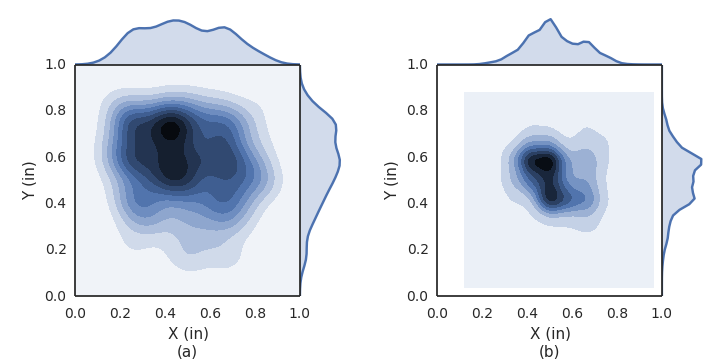
\includegraphics{pe_accuracy.png}
    \caption{Finger press location 2D distribution for (a) HMD, Capacitive, Panel and (b) No HMD, Capacitive, Panel. The distribution is calculated as a Gaussian kernel density estimate. The mean (x, y) location and standard deviation for each is (a) ($0.48\pm0.18, 0.56\pm0.17$) and (b) ($0.52\pm0.12, 0.51\pm0.12$).}
    \label{fig:pe_accuracy}
\end{figure}

A Fitts’ law analysis of the data was not the goal with the experiment design, and since we did not vary the button width a Fitts’ analysis could only be performed with varying distance.
The index of difficulty would only range from 4.0 to 4.5, providing an insufficient range for a proper Fitts’ analysis.
Including extra parameters for the 3D nature of the task \cite{murata_extending_2001, cha_extended_2013} did not improve the fit, especially considering the symmetry of the setup.
Furthermore the time recorded of the tasks were typically more than in a Fitts' task, since many subjects spent time honing based on the accuracy instructions.

%The hand tracker was recording the trajectory in every condition.
%Figure 7 shows representative trajectories of a movement from the left start pad to the top right panel button.
%The button area is shown as a blue box as well on the plots.
%Figure 7(a) shows the trajectory of every subject for HMD, Optical, Panel condition.
%Figure 7(b) focuses on one subject where each line corresponds to each condition.
%This shows a sample of the variation of their trajectory for each condition.
%The plots are both centered at the bottom left corner of the goal button, the z-axis is perpendicular to the button, the y-axis is pointing up from the desk along the panel, and the x-axis is pointed to the right.

%\begin{figure}
%    \centering
%    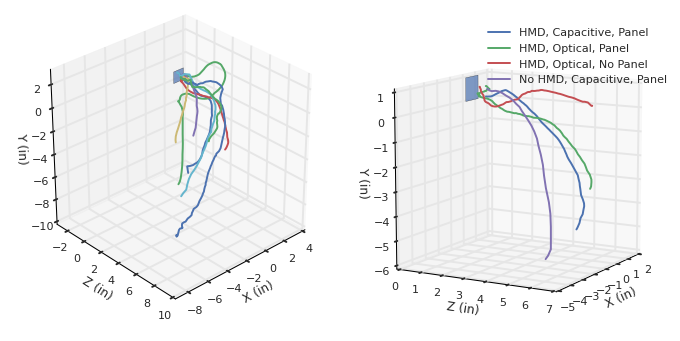
\includegraphics{pe_trajectory.png}
%    \caption{Trajectories of movement for a single trial from left starting pad to top right panel button, for (a) all subjects in HMD, Optical, Panel condition, and (b) one subject, all conditions.}
%    \label{fig:pe_trajectory}
%\end{figure}

\section{Discussion}

The start pads and hand tracker were located relative to each other in such a way that the hand would not be in view of the tracker at the beginning of the task, thus the user would have to wait for the hand tracker to acquire the hand when in view.
This meant for the trials using the HMD the subject would typically have an open loop (blind) ballistic phase followed by the closed loop homing phase once the virtual hand appeared.
Across subjects for all HMD conditions this hand acquisition by the tracker took on average 660ms ($\sigma = 649$ms) from leaving the start pad.
An expert user who performed the experiment was able to get the hand to appear in the tracker in 330ms ($\sigma = 133$ms).
This could indicate that training on how to get the best hand tracker performance could improve results.
The same expert also only experienced a 416ms slowdown between using the HMD and not using the HMD (conditions 1 and 4), compared to the 1.31s slowdown measured across the 8 new subjects.

We had originally hypothesized that having the panel would improve the selection performance of the button, but for this task it had no effect.
This may turn out to be due to the instructions given, which called attention to accuracy.
It is also possible that while the panel did not improve targeting performance in this task, it may provide a benefit to the subjective feeling of presence in the virtual world, which may be beneficial in a more demanding situation with multiple tasks.

Another variable that was not measured was fatigue.
Having the panel as a backstop likely decreases the amount of fatigue for a repeated targeting task, as floating the arm in free space to target a button in a purely virtual environment with no panel can cause a buildup of arm fatigue.
If the virtual world and physical world are correctly aligned, then the finger can rest on the button while the hand tracker works to detect a button press.

Overall, the lack of an effect of having the panel there could also be interpreted as a positive result.
As discussed before, a significant problem we’ve been working on is the improvement of tracking performance when the hand nears the panel.
The results indicate that this problem has been mitigated at least as much to provide performance on par with the purely virtual world.

\section{Future Work}
The promising results from the targeting pilot study indicate that users had no trouble accurately selecting the 1 inch square buttons.
This would be a fairly large button area for an aerospace cockpit.
A future study would investigate the limits of this system in terms of button size, and if smaller buttons pose any significant effect in accuracy.
By varying the button size, this would provide a better experimental design to perform a Fitts’ Law analysis of the R3C system.

As previously discussed, an expert user can handle the inaccuracies of the system better than a novice, thus implying that the pilot study results did not reach an asymptote in training effects, or that there are long term training effects.
The pilot study did not provide any training to subjects so as to not bias a certain condition, but future experiments may include a longer training session before subjects perform tasks in the R3C setup.


\section{Conclusion}

Although this initial application of the R3C system is to aviation/space vehicle cockpits, any sufficiently complex human-system interface could be designed with this system, such as telerobotics, air traffic control, robotic surgery, etc.
The technology that supports our proof of concept system is rapidly improving, and further iterations of our technology integration will provide higher fidelity and an easier user experience.

%\begin{figure}
%    \centering
%    \includegraphics{pe_future.png}
%    \caption{Screenshot from a current demo: User is controlling an external camera on the International Space Station from the cupola.}
%    \label{fig:pe_future}
%\end{figure}

We have showed that new users can accurately select buttons in a simple targeting task in our system.
All of our measured effects showed no significance on correct button selection.
The use of the head mounted display to provide visuals of hand position provides a small time penalty in button selection.
The use of the physical panel provided no significant effect in time compared to having the subjects target purely virtual buttons.
Our optical tracking algorithm had a slight negative effect in time compared to using the capacitive touch sensors.
We are hopeful that training and improvements in the technology will reduce the performance gap.

